\section{Results} % (fold)
\label{sec:pev_results}
%
We applied our method to different stress tensor fields from structural
mechanics simulations.
%
Stress tensors are symmetric tensors that describe the local stress at a point
in a material under acting force.
%
Its eigenvectors are real and orthogonal and are aligned with the principal
stress directions acting on the point.
%
When comparing two different stress tensor fields, \ac{PEV} lines occur where
two principal stress directions align.
%
We show \ac{PEV} lines for three different stress tensor datasets:
%
Two different point loads applied to a uniform material, two different traction
forces applied to the end of a clamped beam, and two different load scenarios
applied to a flange.
%

%
We used the same parameters for all datasets:
%
$\varepsilon_\mathrm{s} = \num{1.e-3}$, $\varepsilon_\mathrm{c} = 5 \times
\varepsilon_\mathrm{s}$, $\varepsilon_\mathrm{d} = \num{1.e-9}$,
$\varepsilon_\mathrm{p} = \num{1.e-3}$.
%
Our results were computed on a 4-core Intel Core i7 \ac{CPU} at
\SI{3.4}{\giga\hertz}.
%
\subsection{Point Loads} % (fold)
\label{ssub:point_loads}
%
\begin{figure}[t]
    \setlength\figurewidth\textwidth
    \centering
    \begin{tikzpicture}[
    every node/.style={node distance=2mm, inner sep=0, outer sep=0},
    image/.style={}
]
    \node[image] (img1) {
        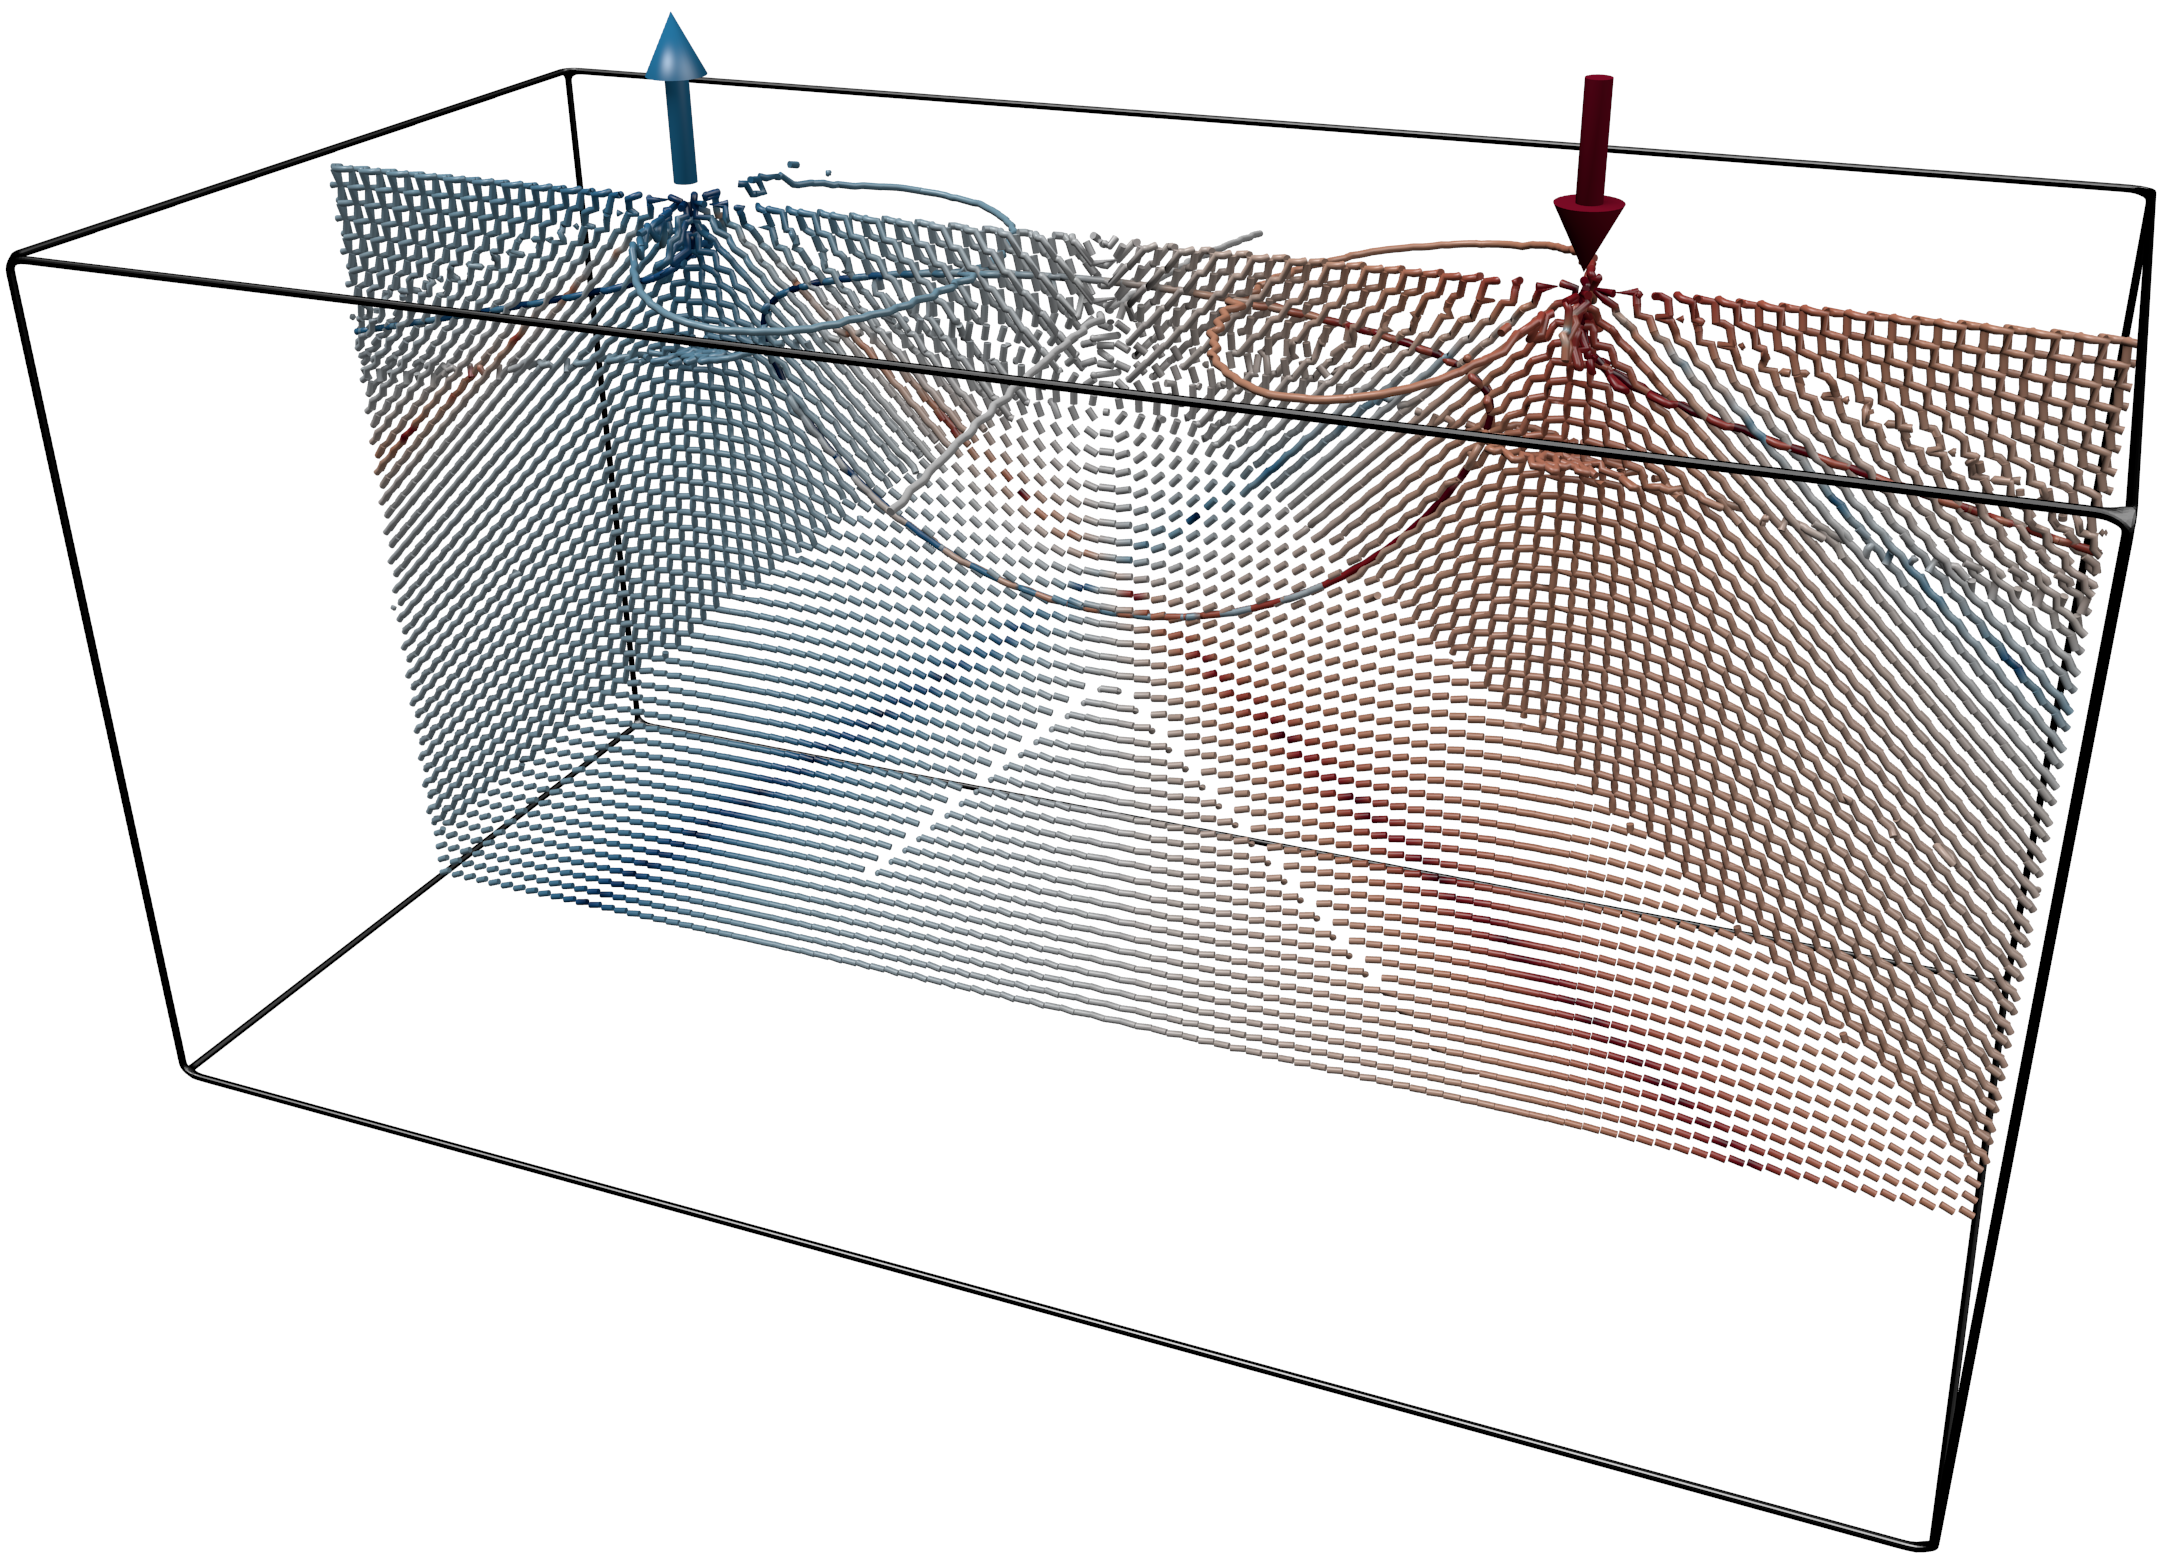
\includegraphics[width=\figurewidth]{figures/PointLoad_total}
    };
    % \begin{scope}[
    %     shift=(img1.south west), % origin is lower left corner
    %     x={($(img1.south east)-(img1.south west)$)}, % x axis is lower side
    %     y={($(img1.north west)-(img1.south west)$)}] % y axis is left side
    %     % \draw[help lines, opacity=0.5, xstep=.01,ystep=.01] (0,0) grid (1,1);
    %     % \draw[thin, xstep=.1,ystep=.1] (0,0) grid (1,1);
    %     % \foreach \x in {0,...,9} { \node [anchor=north] at (\x/10,0) {0.\x}; }
    %     % \foreach \y in {0,...,9} { \node [anchor=east] at (0,\y/10) {0.\y}; }
    %     \draw[mycolor4, thick, rotate around={10:(0.24, 0.81)}]
    %         (0.24, 0.81) ellipse (0.09 and 0.02);
    %     \draw[mycolor4, thick] (0.45, 0.825) circle[radius=5pt];
    %     \draw[mycolor4, thick] (0.51, 0.795) circle[radius=5pt];
    % \end{scope}
    % \node[image, below=of img1.south west, anchor=north west] (img2) {
    %     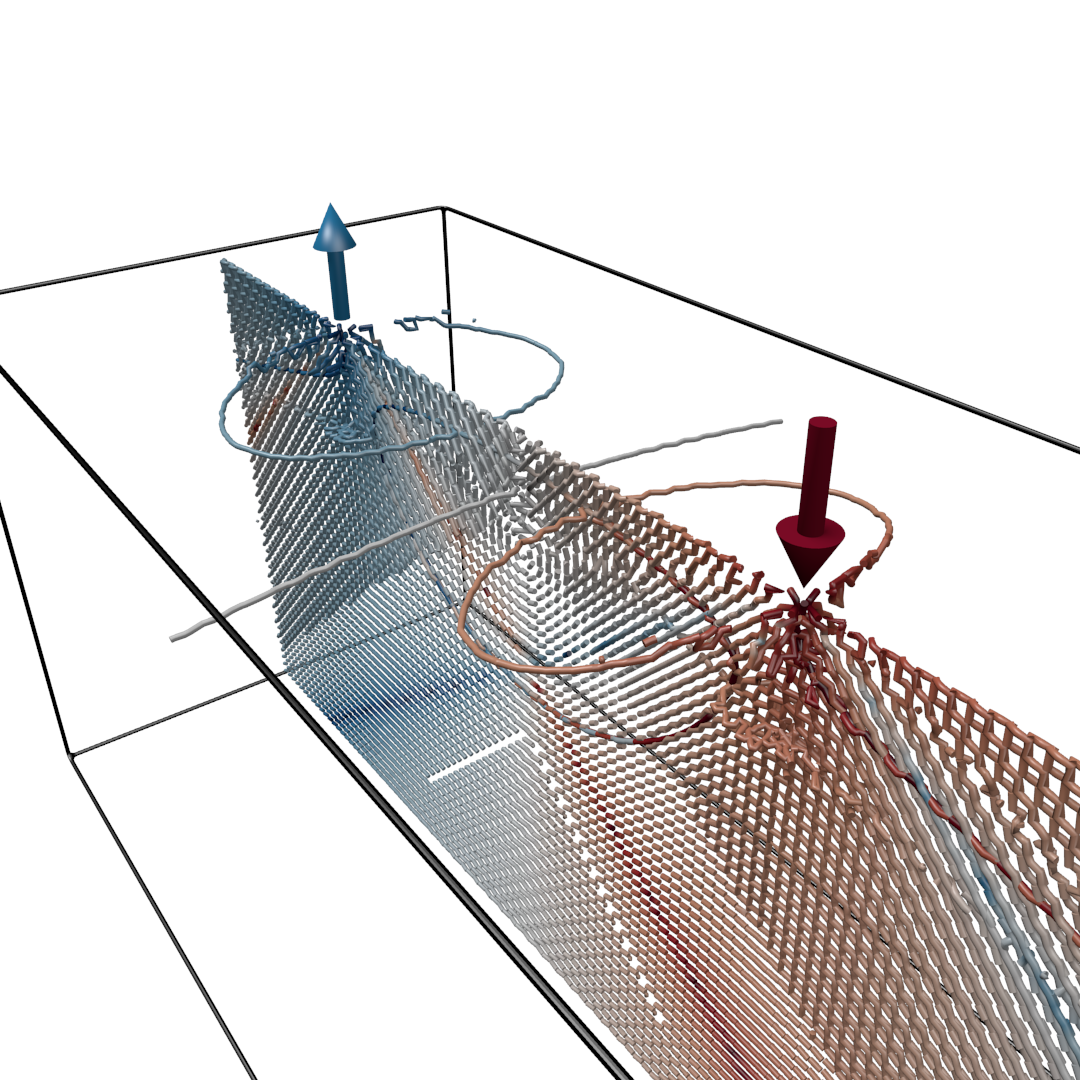
\includegraphics[width=0.5\figurewidth-2mm/2]{figures/PointLoad_detail1_sq}
    % };
    % \begin{scope}[
    %     shift=(img2.south west), % origin is lower left corner
    %     x={($(img2.south east)-(img2.south west)$)}, % x axis is lower side
    %     y={($(img2.north west)-(img2.south west)$)}] % y axis is left side
    %     % \draw[help lines, opacity=0.5, xstep=.01,ystep=.01] (0,0) grid (1,1);
    %     % \draw[thin, xstep=.1,ystep=.1] (0,0) grid (1,1);
    %     % \foreach \x in {0,...,9} { \node [anchor=north] at (\x/10,0) {0.\x}; }
    %     % \foreach \y in {0,...,9} { \node [anchor=east] at (0,\y/10) {0.\y}; }
    %     % \draw[red, thick, rotate around={-45:(0.85, 0.27)}]
    %     %     (0.85, 0.27) ellipse (0.2 and 0.05);
    %     % \draw[red, thick, rotate around={15:(0.62, 0.47)}]
    %     %     (0.62, 0.47) ellipse (0.23 and 0.1);
    %     % \draw[red, thick, rotate around={7:(0.36, 0.64)}]
    %     %     (0.36, 0.64) ellipse (0.19 and 0.08);
    %     % \draw[red, thick, rotate around={20:(0.44, 0.51)}]
    %     %     (0.44, 0.51) ellipse (0.32 and 0.04);
    %     % \draw[red, thick] (0.45, 0.6) circle[radius=5pt];
    %     % \draw[red, thick] (0.5, 0.54) circle[radius=5pt];
    %     % \draw[red, thick] (0.55, 0.53) circle[radius=5pt];
    % \end{scope}
    \node[image, anchor=south west] (img3)
        at (img1.south west) {
        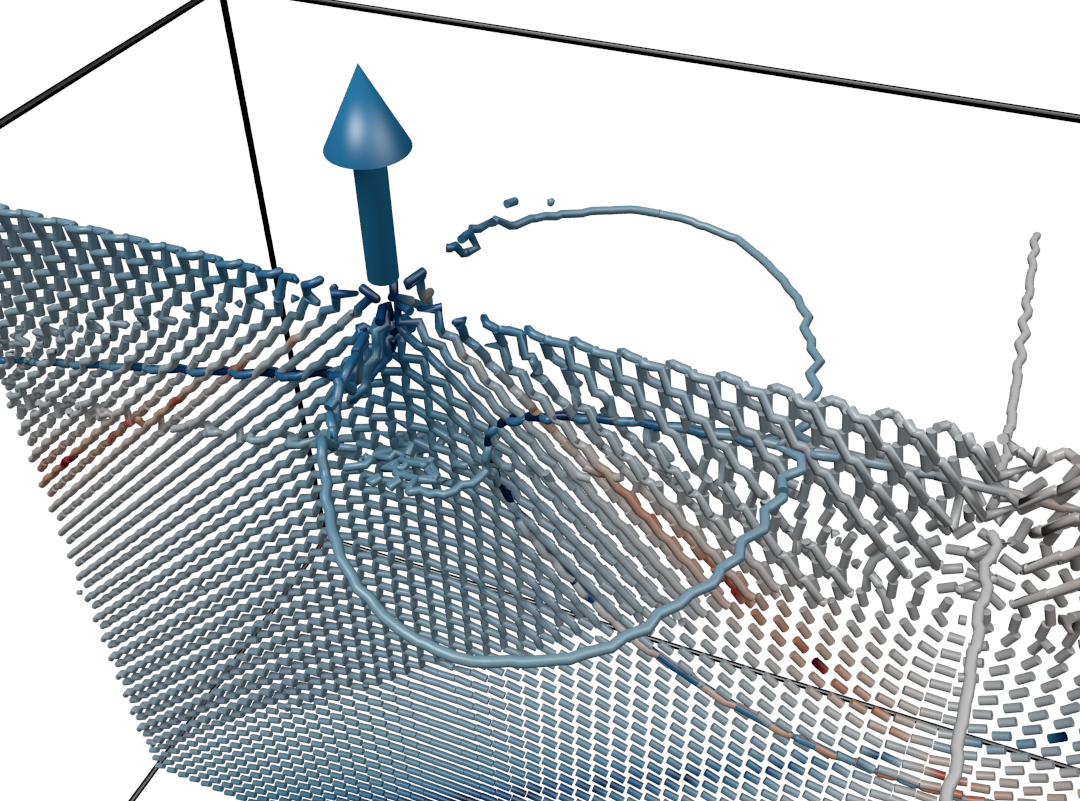
\includegraphics[width=0.5\figurewidth]{figures/PointLoad_detail2}
    };
    \draw[draw=white, line width=3pt]
        (img3.north west) -- (img3.north east) -- (img3.south east);
    \begin{scope}[
        shift=(img3.south west), % origin is lower left corner
        x={($(img3.south east)-(img3.south west)$)}, % x axis is lower side
        y={($(img3.north west)-(img3.south west)$)}] % y axis is left side
        % \draw[help lines, opacity=0.5, xstep=.01,ystep=.01] (0,0) grid (1,1);
        % \draw[thin, xstep=.1,ystep=.1] (0,0) grid (1,1);
        % \foreach \x in {0,...,9} { \node [anchor=north] at (\x/10,0) {0.\x}; }
        % \foreach \y in {0,...,9} { \node [anchor=east] at (0,\y/10) {0.\y}; }
        \draw[mycolor4, thick, rotate around={-2:(0.16, 0.54)}]
            (0.16, 0.54) ellipse (0.15 and 0.02);
        \draw[mycolor4, thick] (0.74, 0.43) circle[radius=5pt];
        \draw[mycolor4, thick] (0.91, 0.35) circle[radius=5pt];
    \end{scope}
\end{tikzpicture}
    \vspace*{-5mm}
    \caption{\ac{PEV} lines for the \textsc{Point Loads} dataset. Lines are
             colored by absolute eigenvalue ratio.}
    \label{fig:point_load}
\end{figure}
%
In this example, we compare two different point loads applied to a uniform
material with infinite extent.
%
The first load (red arrow in \cref{fig:point_load}) is a compressive force,
the second load (blue arrow) is a tensile force of equal magnitude.
%
We compute the \ac{PEV} operator for the two resulting stress tensor fields.
%
The \textsc{Point Loads} case has a closed analytic solution~\cite{Saada2013},
which we sampled on a regular grid with $\num{100} \times \num{50} \times
\num{50}$ points using the \texttt{vtkPointLoad} source from the Visualization
Toolkit~\cite{Schroeder2006}.
%
We then tetrahedralized the data, resulting in \num{1.1} million cells and
\num{4.8} million faces.
%
The computing time for this dataset was \SI{4.2}{\hour}, which means that
\ac{PEV} intersections on each face were found in \SI{3.2}{\milli\second} on
average.
%

%
Since the point loads were applied in the same plane, this synthetic dataset
shows the rare case where eigenvectors are parallel on a plane instead of a
line.
%
This degenerate case also accounts for the long computing time, as for each face
intersected by the \ac{PEV} plane, the recursive subdivision can not be
terminated early.
%
Even though this structurally unstable case produces visual artifacts when
using our method, interesting \ac{PEV} line structures are still visible.
%
There is a bifurcation point exactly at both load points, extending into a
curved ring slightly below the surface.
%
At the second intersection of this ring with the central plane, another closed
\ac{PEV} structure embedded into the plane becomes visible.
%
Within a \ac{PEV} plane, structures where all three eigenvectors are parallel
become lines, instead of points.
%
A similar structure can be observed starting at the load points and leading
outwards.
%
In the center of the dataset, there is another \ac{PEV} line, orthogonal to the
plane and slightly curved downwards, separating the two load points.
%
For this dataset, we colored the \ac{PEV} lines by the absolute eigenvalue ratio
of the parallel eigenvectors.
%
Since both tensor fields result from forces of equal magnitude, this ratio makes
visible the directions in which forces propagate outwards from the load points.
%
% subsubsection point_loads (end)
%
\subsection{Clamped Beam} % (fold)
\label{ssub:clamped_beam}
%
\begin{figure}[t]
    \setlength\figurewidth\textwidth
    \centering
    \begin{tikzpicture}[
    every node/.style={node distance=2mm, inner sep=0, outer sep=0},
    image/.style={}
]
    \node[image] (img1){
        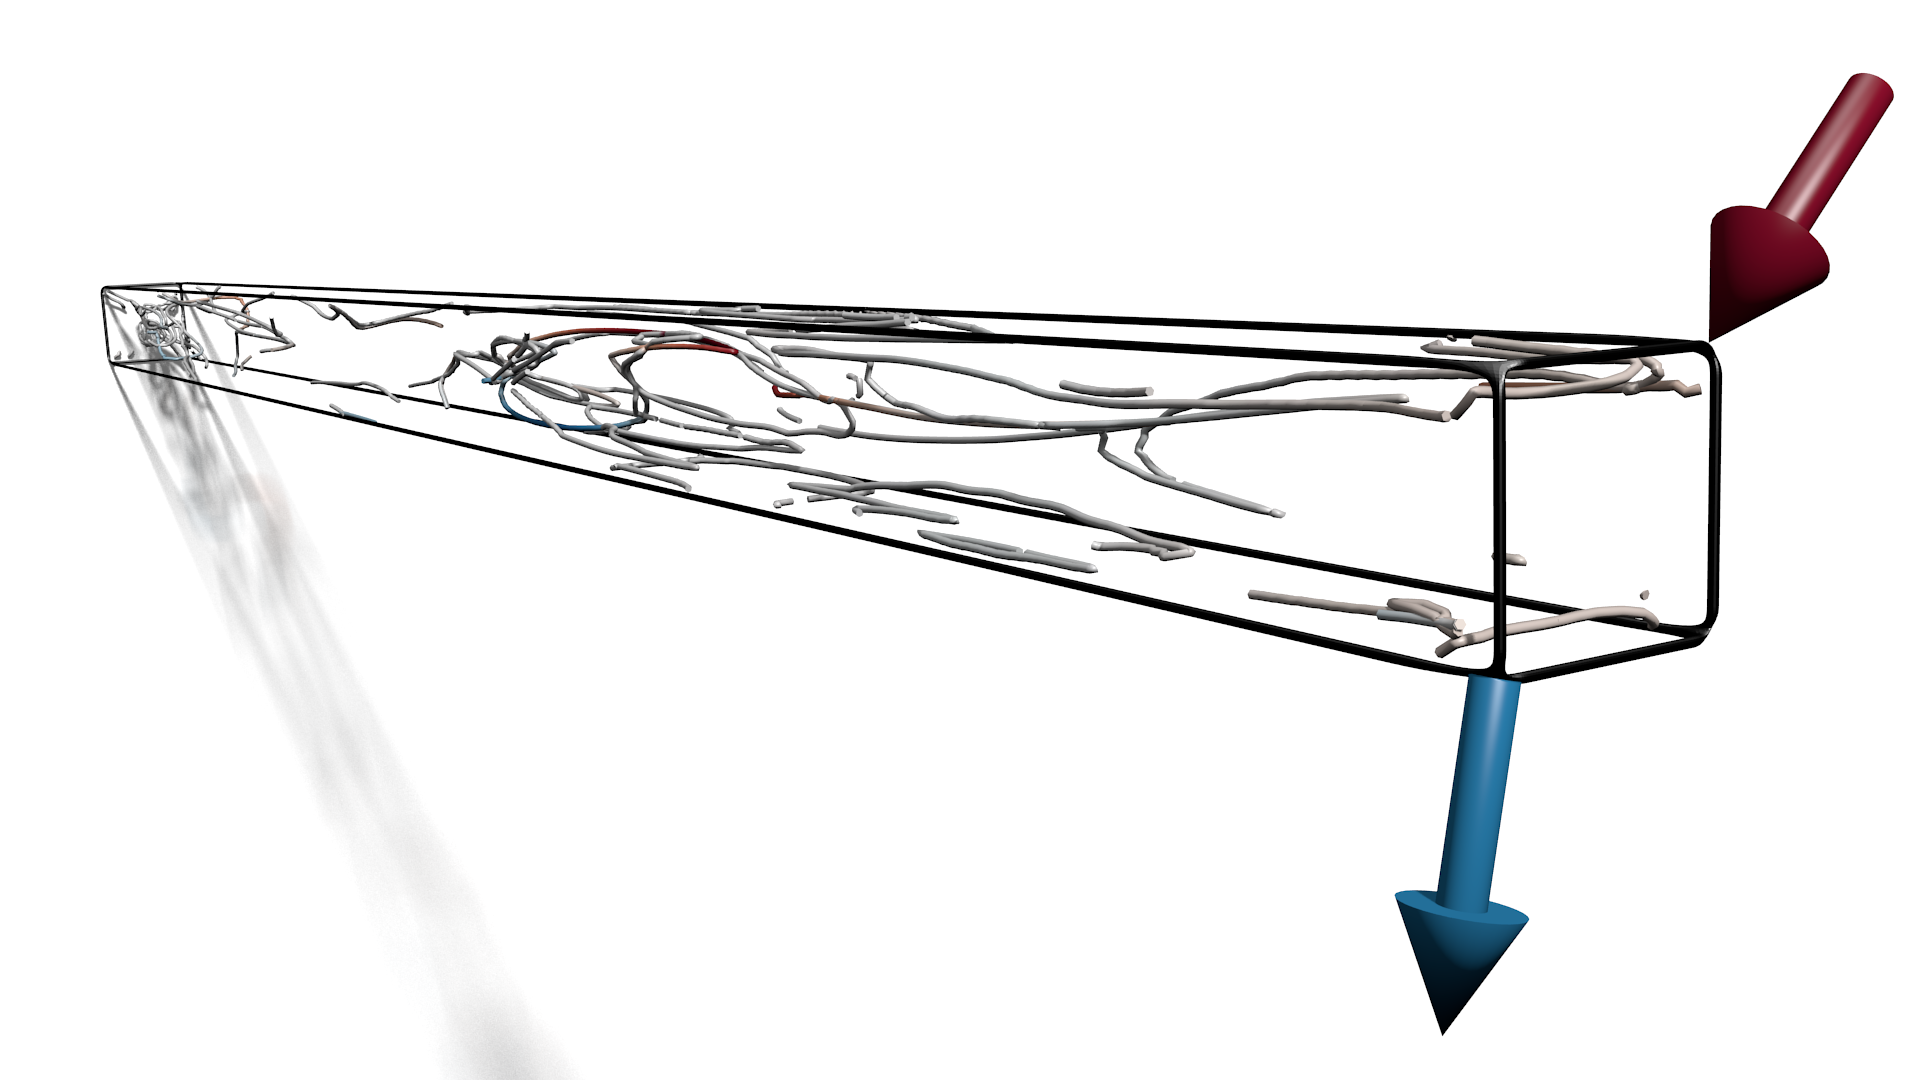
\includegraphics[width=\figurewidth]{figures/beam_full_total}
    };

    \node[image, below=of img1.south west, anchor=north west] (img2) {
        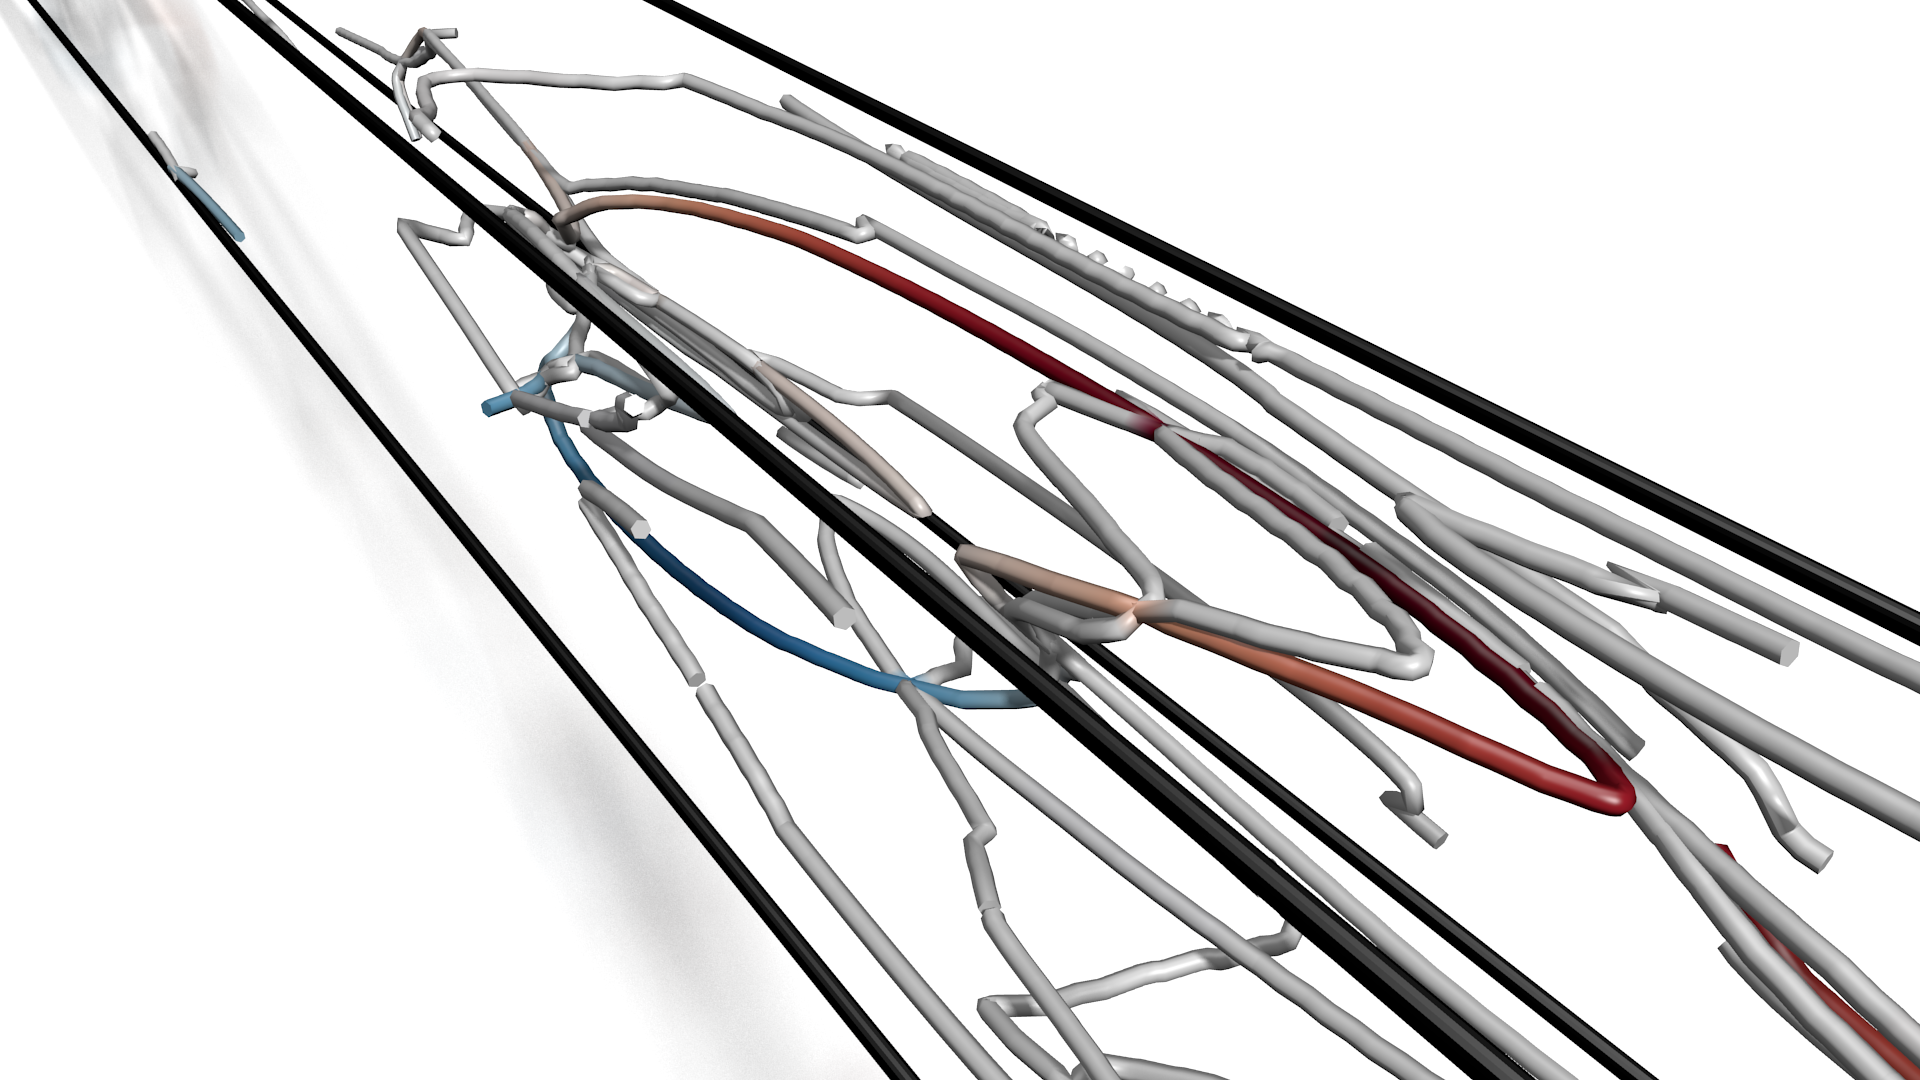
\includegraphics[width=0.5\figurewidth-2mm/2]{figures/beam_full_detail1}
    };
    \begin{scope}[
        shift=(img2.south west), % origin is lower left corner
        x={($(img2.south east)-(img2.south west)$)}, % x axis is lower side
        y={($(img2.north west)-(img2.south west)$)}] % y axis is left side
        % \draw[help lines, opacity=0.5, xstep=.01,ystep=.01] (0,0) grid (1,1);
        % \draw[thin, xstep=.1,ystep=.1] (0,0) grid (1,1);
        % \foreach \x in {0,...,9} { \node [anchor=north] at (\x/10,0) {0.\x}; }
        % \foreach \y in {0,...,9} { \node [anchor=east] at (0,\y/10) {0.\y}; }
        \draw[mycolor4, very thick, rotate around={-25:(0.55, 0.5)}]
            (0.55, 0.5) ellipse (0.35 and 0.25);
    \end{scope}

    \node[image, right=of img2] (img4) {
        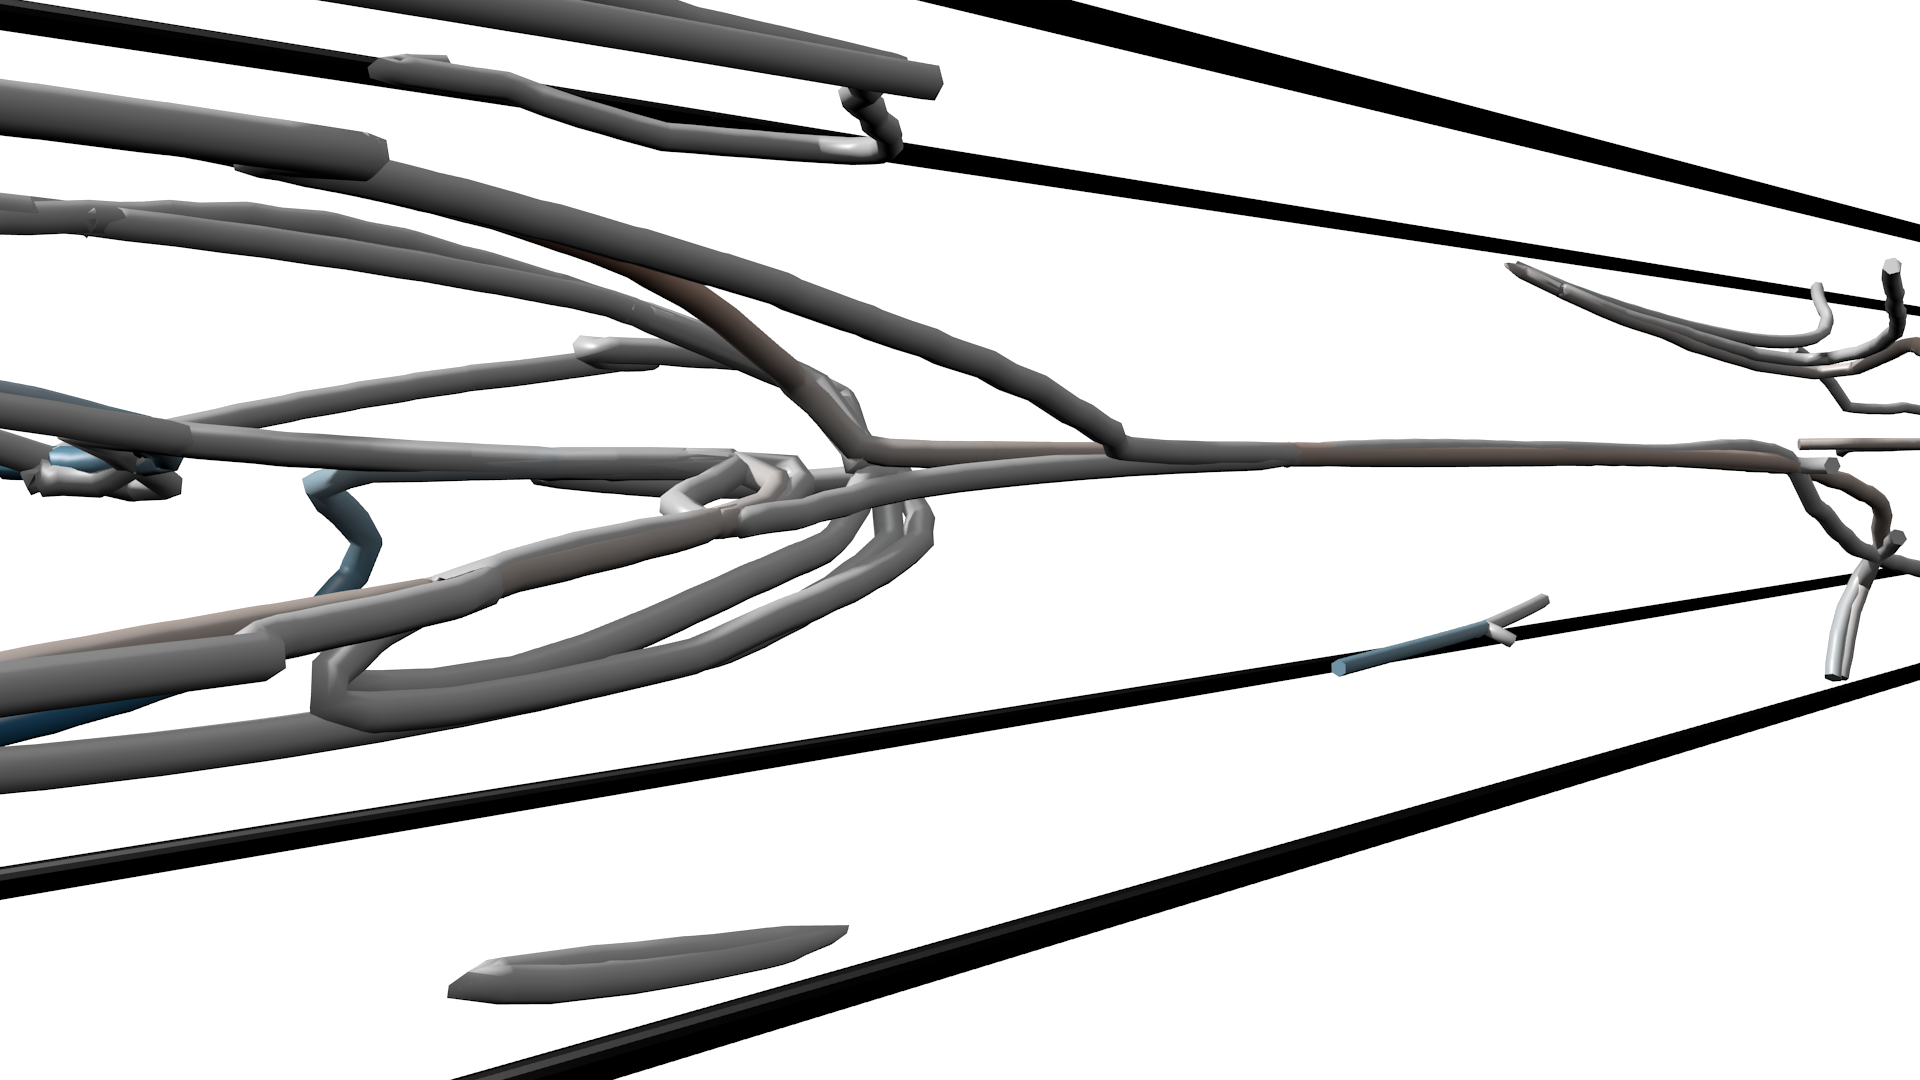
\includegraphics[width=0.5\figurewidth-2mm/2]{figures/beam_full_detail2}
    };
    \begin{scope}[
        shift=(img4.south west), % origin is lower left corner
        x={($(img4.south east)-(img4.south west)$)}, % x axis is lower side
        y={($(img4.north west)-(img4.south west)$)}] % y axis is left side
        % \draw[help lines, opacity=0.5, xstep=.01,ystep=.01] (0,0) grid (1,1);
        % \draw[thin, xstep=.1,ystep=.1] (0,0) grid (1,1);
        % \foreach \x in {0,...,9} { \node [anchor=north] at (\x/10,0) {0.\x}; }
        % \foreach \y in {0,...,9} { \node [anchor=east] at (0,\y/10) {0.\y}; }
        \draw[mycolor4, very thick] (0.75, 0.58) ellipse (0.2 and 0.05);
    \end{scope}
\end{tikzpicture}%
    \caption{\ac{PEV} lines for the \textsc{Clamped Beam} dataset. Lines are
             colored by the eigenvalue of the stress tensor corresponding to the
             red arrow (red is positive, blue is negative). Interesting
             structures mentioned in the text are highlighted.}
    \label{fig:beam_full}
\end{figure}
%
Next, we extracted \ac{PEV} lines for a beam that is fixed on one side.
%
We applied two different traction forces on the free end of the beam, whose
directions are indicated by the blue and red arrows in~\cref{fig:beam_full}.
%
The \textsc{Clamped Beam} dataset consists of \num{150}\si{\kilo} cells and
\num{600}\si{\kilo} faces.
%
The computing time was \SI{26}{\minute}, which means \SI{2.6}{\milli\second}
per face on average.
%

%
% The resulting \ac{PEV} lines are surprisingly complex for such a simple case.
% %
% However, the eigenvalues corresponding to the parallel eigenvectors are near
% zero in a lot of cases, which might mean they exist due to numerical noise.
% %
% Nevertheless, we did not filter them out for rendering, as they showcase nicely
% the high frequency of bifurcation points in symmetric tensor fields.
%

%
There are two regions of particular interest in the \textsc{Clamped Beam}.
%
The first is near the middle of the beam, where a curved structure has high
eigenvalues in both tensor fields (visible in red and blue
in~\cref{fig:beam_full}, bottom left).
%
This is where the beam experiences a lot of stress, and therefore the tensor
fields have a high magnitude.
%
The second is somewhat further towards the wall.
%
Here, all three eigenvector directions are parallel along a line structure near
the center with considerable length (bottom right).
%
This area seems to be the most similar between the two scenarios in terms of
stress directions.
%
% subsubsection clamped_beam (end)
%
\subsection{Flange} % (fold)
\label{ssub:flange}
%
\begin{figure}[p]
    \setlength\figurewidth\textwidth
    \centering
    \begin{tikzpicture}[
    every node/.style={node distance=2mm, inner sep=0, outer sep=0},
    image/.style={}
]
    \node[image] (img1) {
        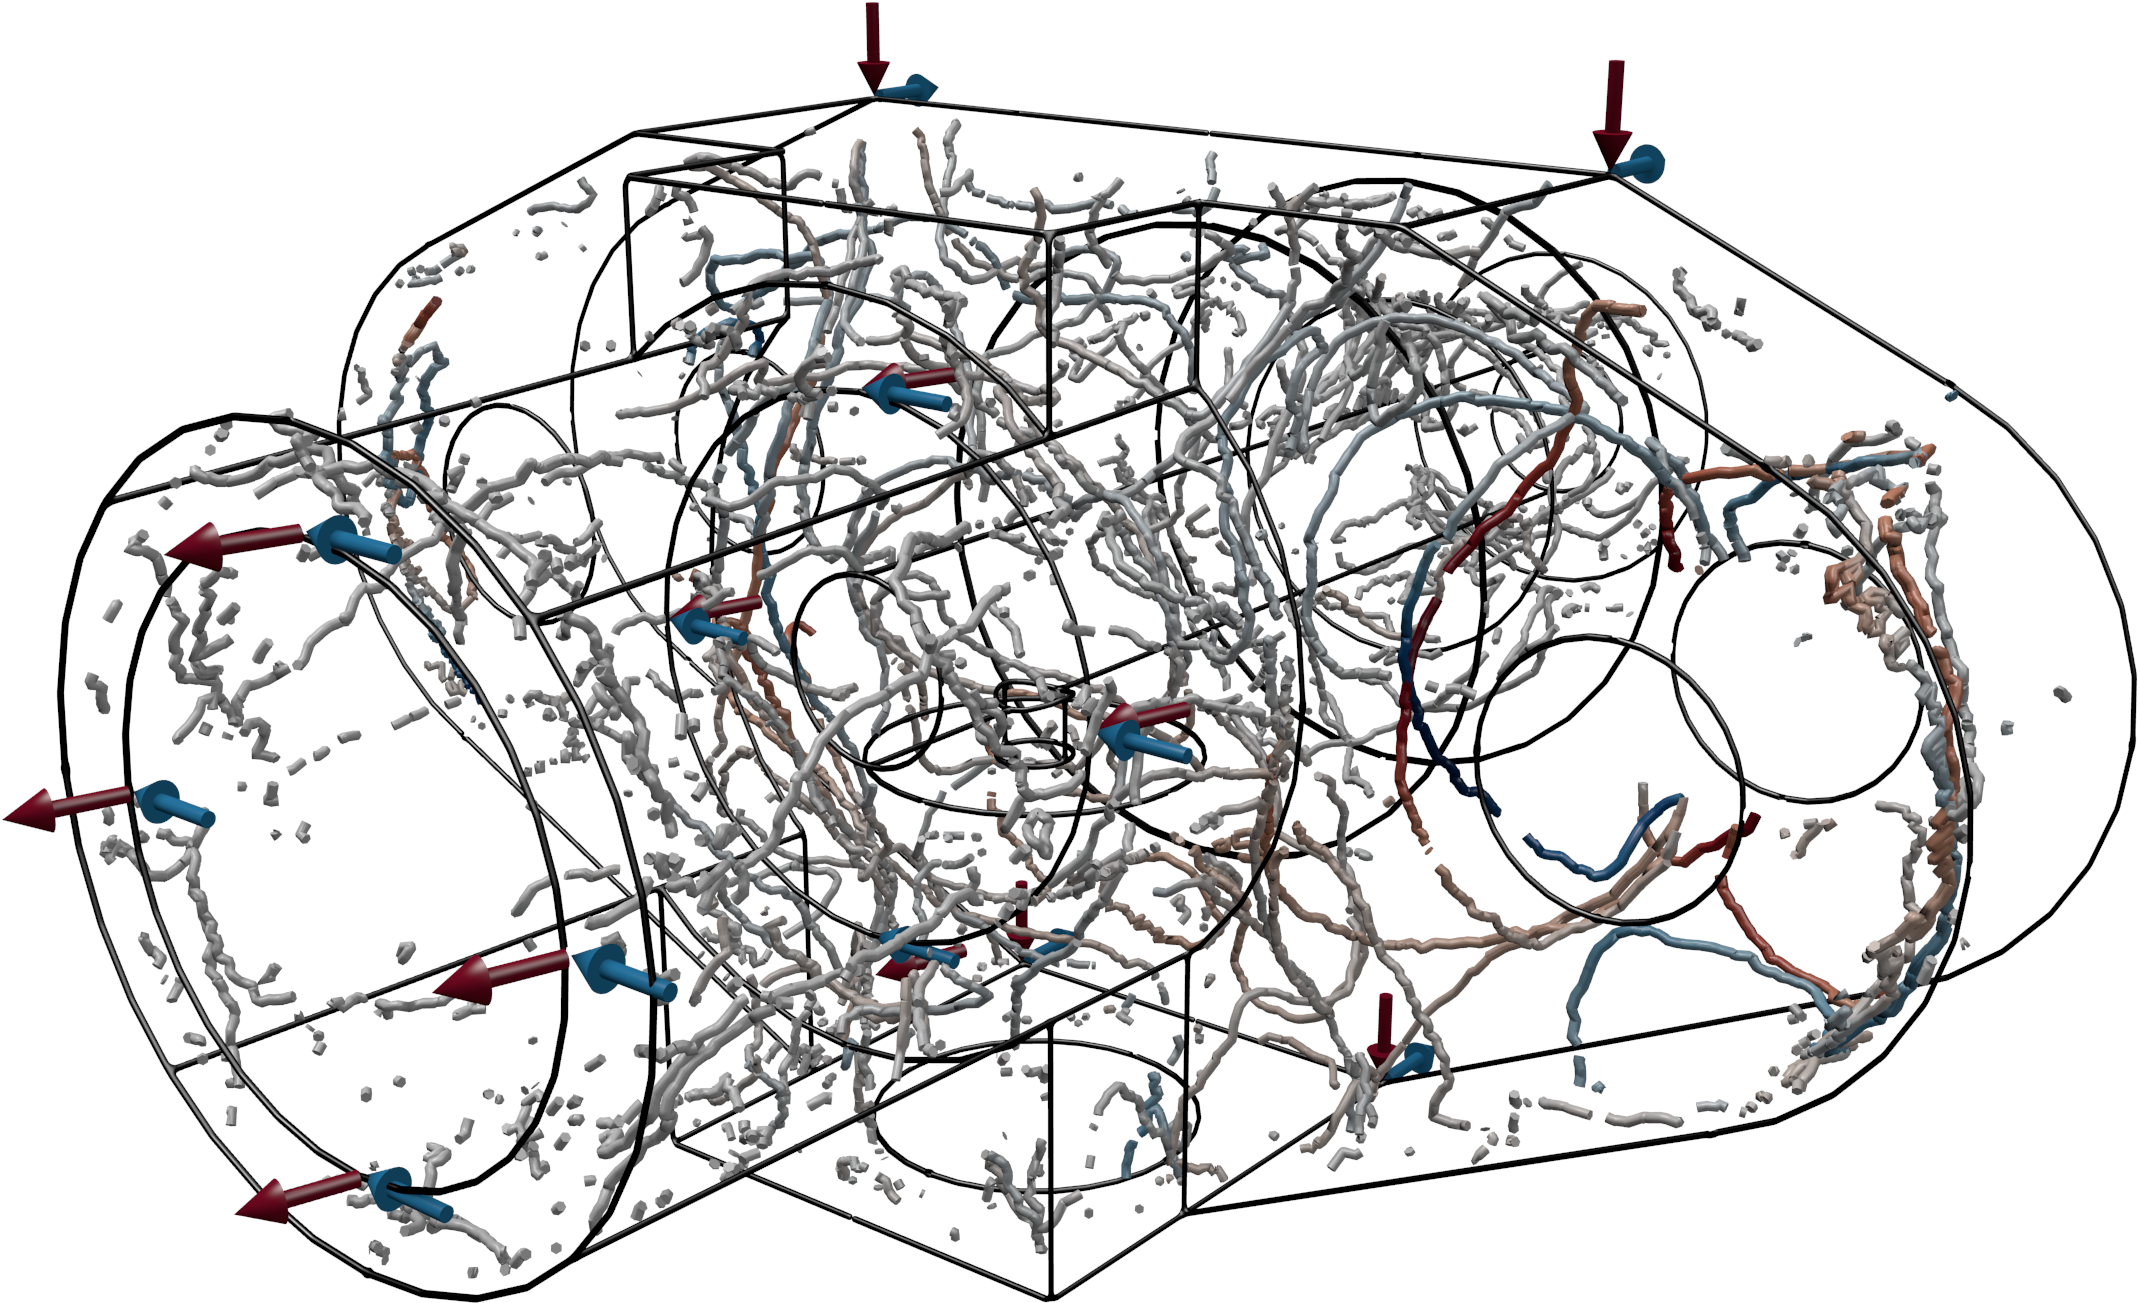
\includegraphics[width=\figurewidth]{figures/flange_full_total}
    };

    \node[image, below=of img1.south west, anchor=north west] (img2) {
        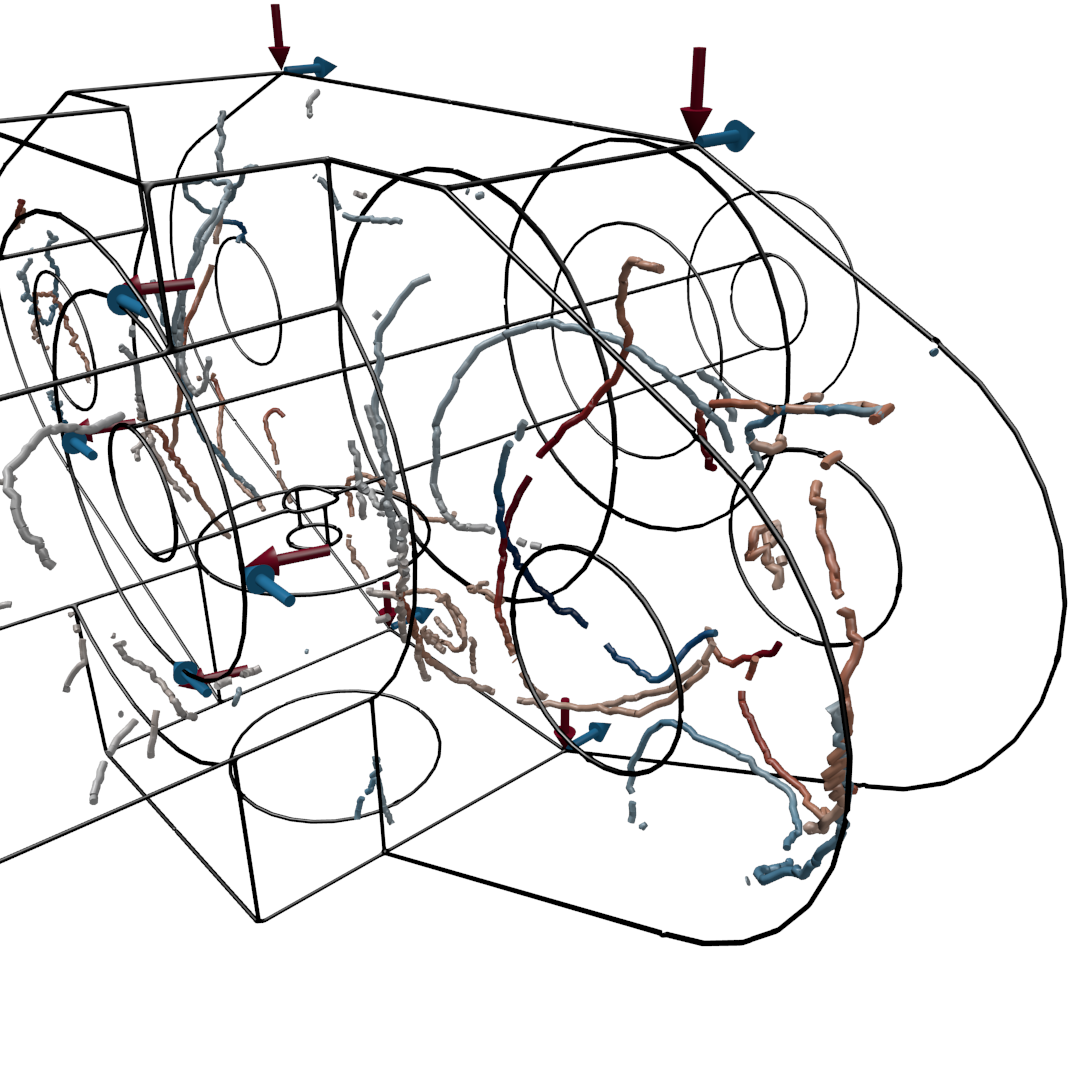
\includegraphics[width=0.5\figurewidth-2mm/2]{figures/flange_detail1_sq}
    };
    \begin{scope}[
        shift=(img2.south west), % origin is lower left corner
        x={($(img2.south east)-(img2.south west)$)}, % x axis is lower side
        y={($(img2.north west)-(img2.south west)$)}] % y axis is left side
        % \draw[help lines, opacity=0.5, xstep=.01,ystep=.01] (0,0) grid (1,1);
        % \draw[thin, xstep=.1,ystep=.1] (0,0) grid (1,1);
        % \foreach \x in {0,...,9} { \node [anchor=north] at (\x/10,0) {0.\x}; }
        % \foreach \y in {0,...,9} { \node [anchor=east] at (0,\y/10) {0.\y}; }
        \draw[mycolor4, very thick] (0.58, 0.68) circle[radius=5pt];
        \draw[mycolor4, very thick] (0.47, 0.5) circle[radius=5pt];
    \end{scope}

    \node[image, right=of img2] (img3) {
        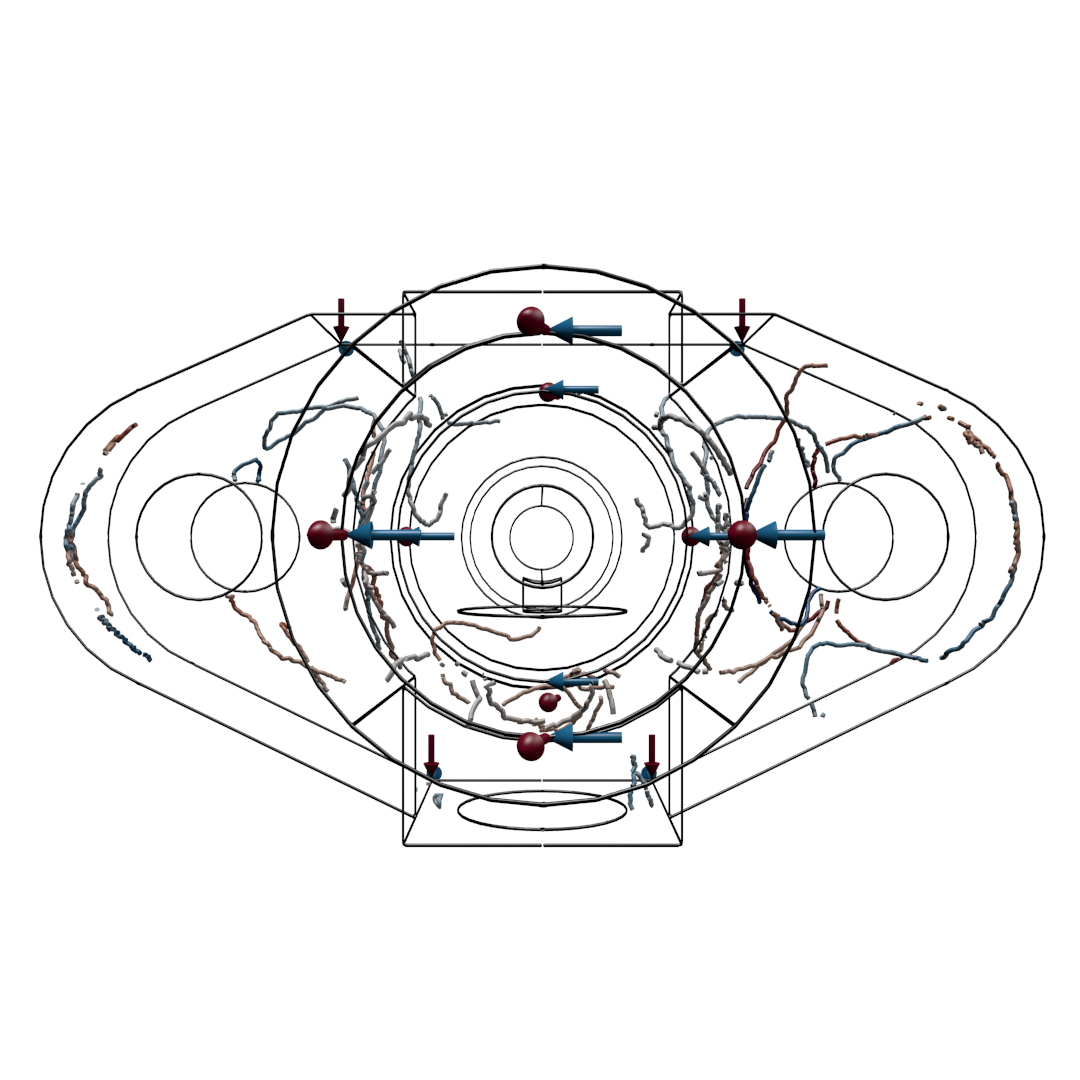
\includegraphics[width=0.5\figurewidth-2mm/2]{figures/flange_detail2_sq}
    };
    \begin{scope}[
        shift=(img3.south west), % origin is lower left corner
        x={($(img3.south east)-(img3.south west)$)}, % x axis is lower side
        y={($(img3.north west)-(img3.south west)$)}] % y axis is left side
        % \draw[help lines, opacity=0.5, xstep=.01,ystep=.01] (0,0) grid (1,1);
        % \draw[thin, xstep=.1,ystep=.1] (0,0) grid (1,1);
        % \foreach \x in {0,...,9} { \node [anchor=north] at (\x/10,0) {0.\x}; }
        % \foreach \y in {0,...,9} { \node [anchor=east] at (0,\y/10) {0.\y}; }
        \draw[mycolor4, very thick] (0.75, 0.6) circle[radius=10pt];
        \draw[mycolor4, very thick] (0.75, 0.4) circle[radius=10pt];
    \end{scope}
\end{tikzpicture}
    \caption{\ac{PEV} lines for the \textsc{Flange} dataset. Lines are colored
             by the eigenvalue corresponding to the red arrows. The top image
             shows all lines while the bottom shows only lines where the
             magnitudes of both eigenvalues are above a threshold. Interesting
             structures mentioned in the text are highlighted.}
    \label{fig:flange_filtered}
\end{figure}
%
% 1.2 million cells
%
% 5 million faces
%
% Computing time: \SI{36}{\minute}
%
% Time per face: \SI{0.45}{\milli\second}
%
Our final stress tensor dataset is a flange from an OpenFoam~\cite{OpenFOAMWWW}
tutorial.
%
We subjected the flange to two different loads, applied on the back wall and the
flange ring (see red and blue arrows in \cref{fig:flange_filtered}).
%
The original mesh uses polygonal cells, which is why we resampled the data,
resulting in \num{1.2} million cells and \num{5} million faces.
%
The computing time was \SI{36}{\minute}, \ie{}, \SI{0.5}{\milli\second} per face.
%

%
The \textsc{Flange} dataset exhibits a lot of \ac{PEV} lines, which can be seen
in~\cref{fig:flange_filtered} (top).
%
Most of the \ac{PEV} lines correspond to eigenvectors with small eigenvalues in
both tensor fields.
%
We therefore filtered out all \ac{PEV} lines where both eigenvalues are very
small in the bottom images in~\cref{fig:flange_filtered}.
%
Especially prominent are two bifurcation points with high eigenvalues between
the two outer screw holes and the central tube (bottom left).
%
There are also \ac{PEV} lines leading outwards both above and below the screw
holes (bottom right).
%
In general, the most similar directions of significant stress are near the screw
holes and in the area where the large flange ring meets the central block.
%
% subsubsection flange (end)
%
% subsection stress_tensor_data (end)
%
% section results (end)